\documentclass[aps,prb,twocolumn,superscriptaddress,floatfix,longbibliography]{revtex4-2}
\usepackage{graphicx}
\usepackage{amsmath,amssymb,amsthm}
\usepackage{bm}
\usepackage{xcolor}
\usepackage[colorlinks=true,linkcolor=blue!60!black,citecolor=blue!60!black,urlcolor=blue!60!black]{hyperref}

\newtheorem{theorem}{Theorem}
\newtheorem{proposition}{Proposition}
\newtheorem{lemma}{Lemma}
\newtheorem{conjecture}{Conjecture}
\newcommand{\eps}{\varepsilon}
\newcommand{\ave}[1]{\langle #1\rangle}
\newcommand{\floor}[1]{\lfloor #1\rfloor}

\begin{document}

\title{Boundary-controlled algebraic vorticity order in Shakti artificial spin ice}

\author{Changyeon Won}
\email{cywon@khu.ac.kr}
\affiliation{Department of Physics, Kyung Hee University, Seoul 02447, Republic of Korea}

\date{\today}

\begin{abstract}
In the ground states of Shakti artificial spin ice every unhappy vertex joins two perpendicular rectangular plaquettes into an L-shaped tetromino, so that the ground states correspond one-to-one to domino tilings. We show that the circulation of the island moments around each tetromino, a vorticity $v=\pm1$, is a hidden collective variable with a rigid structure. It is an explicit function of the dimer height field, $v=s(-1)^{\floor{h/4}}$ with a fixed period-4 prefactor $s$; consequently the island coupling rule is never frustrated, $v$ is unique up to a global sign, and the total vorticity is a topological invariant given by a closed formula in terms of boundary data. Inside the sample $v$ forms a $2\times2$ superstructure with algebraic order whose amplitude decays as $L^{-1/4}$. We establish this with exact Kasteleyn calculations and find a conjectured product formula for the amplitude at the center of an Aztec-diamond sample, with asymptotic constant $e^{1/4}2^{1/3}A^{-3}$, where $A$ is the Glaisher constant. All vorticity patterns are projections of a single phase field $\Psi\simeq e^{i\pi\langle h\rangle/4}$ set by the mean height, so the sample boundary selects which plaquette orientation orders and with which sign; at the sample center the phase is fixed exactly by symmetry. The order produces power-law superlattice peaks in the structure factor, with heights $\propto L^{3/2}$ and $|\bm q-\bm q_0|^{-3/2}$ tails. Point defects are classified by their winding: half vortices are confined by strings of violated couplings, whereas full vortices are free and screen the order. Dipolar interactions preserve the algebraic phase down to $T_c\approx0.45D$, below which a flat crystal with long-range vorticity order forms. The results provide rules for designing and reading out vorticity order in nanomagnet arrays.
\end{abstract}

\maketitle

%==========================================================================
\section{Introduction}
%==========================================================================

Artificial spin ices are arrays of elongated single-domain nanomagnets whose moments behave as Ising spins pinned to the edges of a lattice~\cite{Wang2006,Nisoli2013RMP,Skjaervo2020}. Because the lattice geometry can be chosen at will and every moment can be imaged, they have become a laboratory for frustration, emergent gauge fields, and magnetic charges~\cite{Moller2006,Castelnovo2008,Henley2010,Perrin2016,Farhan2013}. In the square and kagome geometries frustration lives at the vertices, and the low-energy physics is controlled by an ice rule. A second route, \emph{vertex frustration}, was opened by lattices in which not all vertices can simultaneously reach their lowest-energy configuration~\cite{Morrison2013}. The best studied example is the Shakti lattice~\cite{Chern2013,Gilbert2014,Lao2018}. Its minimal loops are rectangular plaquettes, and in every ground state each plaquette contains exactly one ``unhappy'' three-leg vertex that it shares with a neighboring, perpendicular plaquette. The unhappy vertices therefore form a dimer covering of the square lattice of plaquettes, which explains the extensive degeneracy, the emergent ice rule, and the classical topological order observed in Shakti arrays~\cite{Chern2013,Gilbert2014,Lao2018}.

The dimer description tells us \emph{where} the frustration sits, but it does not say which collective magnetic pattern the arrays actually display. In the present work we identify such a pattern. We regard each dimer together with its two plaquettes as an L-shaped tetromino (Fig.~\ref{fig:mapping}). The ten islands on the perimeter of a tetromino nearly close a flux loop: nine point along a common sense of circulation and one, the \emph{defect island}, points against it. The tetromino thus carries a vorticity $v=\pm1$ (counterclockwise or clockwise), a natural observable in nanomagnet arrays where flux closure is energetically favored and directly imaged. We ask how these vorticities are organized globally, how the sample boundary controls them, and what happens under realistic interactions and defects.

Our main findings are as follows.

\emph{Vorticity is slaved to the height field.} The tetromino vorticity is an explicit local function of the Thurston height of the dimer covering (Sec.~\ref{sec:height}). As a consequence the island coupling rule between tetrominoes is never frustrated, the vorticity of every tetromino is fixed once the tiling is fixed, and the total vorticity $V=\sum v$ is conserved by all local rearrangements. $V$ is a topological invariant of the sample, and we give it in closed form in terms of the boundary alone.

\emph{Algebraic, boundary-imprinted order.} Averaged over the degenerate ground states, $v$ forms a $2\times2$ superstructure whose amplitude decays as $(\text{size})^{-1/4}$ (Sec.~\ref{sec:order}). The exponent follows from the Gaussian free field description of dimers~\cite{Kenyon2001}; we confirm it with exact Kasteleyn calculations and find a closed product formula for the central amplitude of the Aztec-diamond sample.

\emph{One phase field controls all patterns.} All observed $\langle v\rangle$ patterns are projections of a single complex field $\Psi$ whose phase is $\pi\langle h\rangle/4$ (Sec.~\ref{sec:phase}). Sample size modulo 4 and the way the sample is cut from the lattice therefore decide whether the horizontal plaquettes, the vertical plaquettes, or both carry the order; at the sample center the phase is fixed exactly by symmetry. Holes and pinned regions act as additional boundaries that reinforce or twist the pattern.

\emph{Experimental fingerprints, defects, and temperature.} The order gives power-law superlattice peaks in the magnetic structure factor (Sec.~\ref{sec:corr}). Point defects of the tiling fall into two topological classes: half vortices, which are confined by strings, and full vortices, which are free and screen the order (Sec.~\ref{sec:defects}). Point-dipolar and dumbbell interactions leave the algebraic phase intact over a wide temperature window and eventually lock the height into a crystal with true long-range vorticity order (Sec.~\ref{sec:dipolar}). Section~\ref{sec:design} condenses the results into design rules, and Sec.~\ref{sec:conclusion} concludes. Proofs and methods are collected in the Appendices.

%==========================================================================
\section{From Shakti ground states to domino tilings}
\label{sec:mapping}
%==========================================================================

\subsection{Tetrominoes and dominoes}

We use the Shakti lattice in the form of a basketweave of $1\times2$ rectangular plaquettes: $2\times2$ blocks made of two parallel plaquettes, with the block orientation alternating like a checkerboard. Islands sit on the unit edges, except on the middle edge of each plaquette, which is absent. Vertices have coordination $z=2$, 3, or 4.

In a ground state every plaquette contains one unhappy $z=3$ vertex, located at the corner where it touches a perpendicular plaquette~\cite{Morrison2013,Chern2013,Lao2018}. Pairing each plaquette with the plaquette that shares its unhappy vertex gives an L-shaped tetromino made of four unit squares. We map every plaquette to a chessboard cell: horizontal plaquettes to black cells and vertical plaquettes to white cells, such that orthogonally adjacent cells correspond to perpendicular plaquettes that share an edge. The chessboard translations $(2,2)$ and $(2,-2)$ act on the Shakti lattice as translations by $(0,4)$ and $(4,0)$, so the map is a $45^\circ$ rotation with a factor $\sqrt2$, fixed by a fundamental domain of eight cells (Appendix~\ref{app:proofs}). Each cell $c$ also has a diagonal partner $p(c)$, the parallel plaquette in the same block. Under this map a tetromino is a domino and a Shakti ground state is a domino tiling of the corresponding region [Figs.~\ref{fig:mapping}(a) and \ref{fig:mapping}(b)]. The dimer map of Lao \emph{et al.}~\cite{Lao2018} is the same correspondence written for the unhappy vertices; here it is lifted to the level of tiles.

The two plaquettes of a tetromino are inequivalent. The \emph{strong} (short) arm contains the elbow square of the L; the other is the \emph{weak} (long) arm. In chessboard terms the strong cell of the domino $\{x,y\}$ is $y$ if $y$ is orthogonally adjacent to $p(x)$ and $x$ otherwise.

\begin{figure*}[t]
\centering
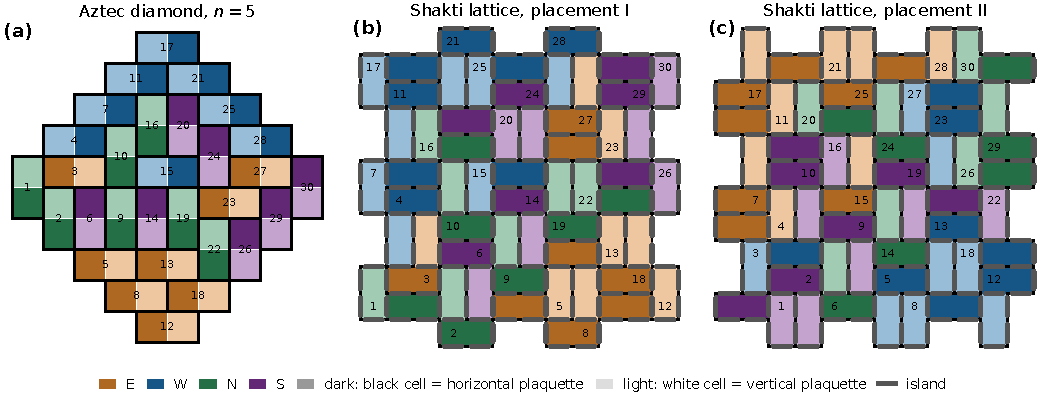
\includegraphics[width=\textwidth]{figs/fig1_mapping.pdf}
\caption{Domino tilings and Shakti ground states. (a) A domino tiling of the Aztec diamond of order $n=5$. Colors label the four domino types (E, W, N, S: position of the white cell relative to the black cell); dark and light shades mark black and white cells. (b) The corresponding L-tetromino tiling of the Shakti lattice in placement I. Gray bars are the nanoislands. Black cells map to horizontal plaquettes and white cells to vertical plaquettes, and each domino becomes an L made of two perpendicular plaquettes that share the unhappy vertex. (c) The same tiling in placement II, where the diamond is shifted by one cell relative to the plaquette blocks. The chessboard coloring, and therefore the domino types and plaquette orientations, change between the two placements; the numbers identify the same domino in all panels.}
\label{fig:mapping}
\end{figure*}

\subsection{Tetromino template, vorticity, and the island rule}

Figure~\ref{fig:template} shows the island configuration of a single tetromino in a ground state. All ten perimeter islands are fixed. Nine of them point along a common circulation, which defines the vorticity $v=+1$ (counterclockwise) or $v=-1$ (clockwise); the tenth, the defect island, points against it. Its position is fixed by the shape: it lies on the weak arm, on the long side facing away from the block partner, on the unit segment next to the elbow. With this template all $z=4$ vertices are of type I and all $z=3$ vertices carry charge $\pm1$. The clockwise state is the time reverse, and the mirror-image (J) tetromino is obtained by reflection. The template also fixes several islands just outside the tetromino.

Two tetrominoes that share an island must agree on its orientation. Since counterclockwise circulations of two adjacent tiles traverse their common edge in opposite directions, this gives a simple rule.

\begin{lemma}[Island rule]
Two tetrominoes that share an island have opposite vorticity, unless the shared island is the defect island of one of them, in which case they have the same vorticity. Two defect islands never coincide.
\end{lemma}

In particular, strong arms never carry a defect island, so tetrominoes in contact through their strong arms always have opposite vorticities, as do block partners (parallel weak arms). The externally fixed islands add further couplings between tiles that touch only at a corner; all of them favor equal vorticities and are consistent with the rule (checked for all 576 relative placements).

\begin{figure*}[t]
\centering
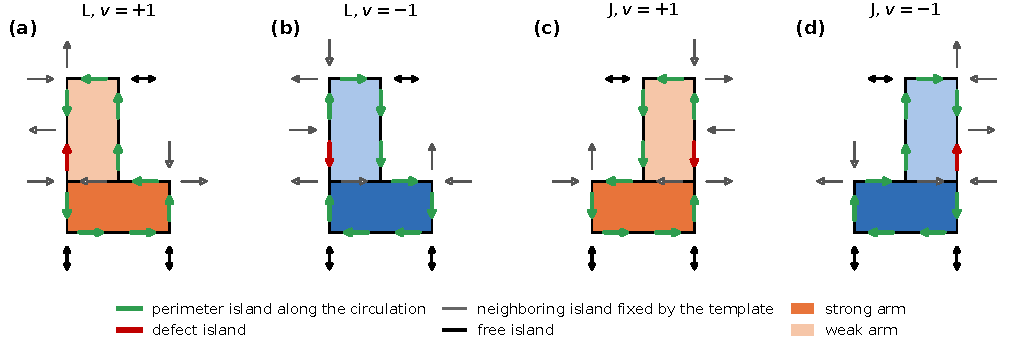
\includegraphics[width=\textwidth]{figs/fig2_template.pdf}
\caption{Island template of a tetromino in a Shakti ground state, for both chiralities (L and J) and both vorticities. Green arrows are perimeter islands along the circulation, and the red arrow is the defect island, which points against it. Open arrows are islands just outside the tile that the template also fixes; double arrows are islands left free. Dark (light) shading marks the strong (weak) arm.}
\label{fig:template}
\end{figure*}

\subsection{Sample geometries}

Artificial spin ices are finite samples, and their boundaries turn out to matter. We consider three families of samples: (a) the Aztec diamond of order $n$, the cell set $|i+\tfrac12|+|j+\tfrac12|\le n$, which is the classic setting for dimers with a frozen boundary and an arctic circle~\cite{EKLP1992,Jockusch1998,Cohn1996}; (b) $L\times L$ square and $W\times H$ rectangular boards; (c) arbitrary simply connected shapes, with or without holes. An Aztec diamond can be cut from the Shakti lattice in two inequivalent ways (placements I and II), which differ by a one-cell shift of the chessboard relative to the plaquette blocks [Figs.~\ref{fig:mapping}(b) and \ref{fig:mapping}(c)]; for square boards the analogue is the color of the corner cell. Since any shape can be fabricated lithographically, we treat all placements on an equal footing.

%==========================================================================
\section{Vorticity as a function of the height field}
\label{sec:height}
%==========================================================================

\subsection{Height formula}

The Thurston height $h$ of a domino tiling lives on the lattice vertices~\cite{Thurston1990}. Along an edge that is not crossed by a domino, $h$ increases by $1$ if the cell to the left is black and decreases by $1$ otherwise; across a domino it changes by $\mp3$. We fix the additive constant so that $h(x,y)\equiv r(x,y)\pmod 4$, with $\bar x=x\bmod 2$, $\bar y=y\bmod2$, and
\begin{equation}
r(x,y)=\bigl[2+\bar x-\bar y+2\bar x\bar y\bigr]\bmod 4 .
\label{eq:residue}
\end{equation}

\begin{proposition}[Height formula]
Let $d$ be a domino whose lower-left cell has lower-left corner $p_d=(x,y)$. Up to one global sign,
\begin{equation}
v(d)=s(d)\,(-1)^{\floor{h(p_d)/4}},
\label{eq:vformula}
\end{equation}
where $s$ depends only on the orientation of $d$ and on $(x\bmod4,\,y\bmod4)$:
\begin{equation}
\begin{aligned}
s_{\rm H}(x,y)&=-(-1)^{\floor{(x+1)/2}+\floor{(y+1)/2}},\\
s_{\rm V}(x,y)&=s_{\rm H}(x,y)\,(-1)^{\bar x\bar y}.
\end{aligned}
\label{eq:sfactor}
\end{equation}
\end{proposition}

Because $h(p_d)\bmod 4$ is fixed by position, the factor $\eps(p)\equiv(-1)^{\floor{h(p)/4}}$ records a single bit of the height field, namely which of the two allowed values of $h\bmod 8$ occurs at $p_d$. The vorticity pattern is therefore a fixed period-4 background multiplied by one bit of the height. The formula was found from all 32\,768 tilings of the $n=5$ Aztec diamond and is proven for every tiling of every region in Appendix~\ref{app:proofs}. Figure~\ref{fig:examples} shows the resulting vorticities for individual tilings together with their averages.

\begin{figure*}[t]
\centering
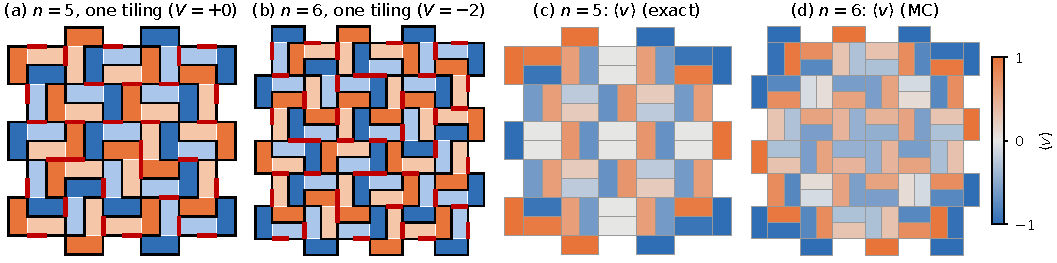
\includegraphics[width=\textwidth]{figs/fig3_examples.pdf}
\caption{Vorticity of individual ground states and its average (Aztec diamond, placement I). (a), (b) One tiling each for $n=5$ and $n=6$, with $v$ obtained from the island rule; orange (blue) is $v=+1$ ($-1$), dark (light) shading the strong (weak) arm, and red bars mark the defect islands. The total vorticity $V$ given in brackets is the same for all tilings of a sample. (c) Average $\langle v\rangle$ per plaquette, exact over all 32\,768 tilings for $n=5$. (d) The same for $n=6$ from $2\times10^4$ samples.}
\label{fig:examples}
\end{figure*}

\subsection{No frustration and uniqueness}

Equation~\eqref{eq:vformula} satisfies every coupling of the island rule, including the corner couplings, in every tiling of every simply connected region (Lemma~\ref{lem:local} in Appendix~\ref{app:proofs}). The coupling network is thus never frustrated. Moreover, any two edge-adjacent dominoes share a perimeter island, so the coupling graph contains the adjacency graph of the tiling and is connected. The vorticity of each tetromino is therefore uniquely determined by the tiling, up to one global sign that the boundary fixes. The vorticity is not an extra degree of freedom on top of the dimers; it is a nonlocal functional of the dimer configuration, carried by the height field.

\subsection{Conservation of the total vorticity}

A $2\times2$ flip of two parallel dominoes changes $h$ only at the center of the block, which is the reference vertex $p_d$ of no domino. By Eq.~\eqref{eq:vformula} only the two flipped tetrominoes change, and a direct evaluation shows that their sum does not (Appendix~\ref{app:proofs}, Fig.~\ref{fig:flip}): blocks whose lower-left cell has $x+y$ even carry opposite vorticities before and after the flip, blocks with $x+y$ odd carry equal ones of the same sign. Since all tilings of a simply connected region are connected by flips~\cite{Thurston1990}, we obtain the following.

\begin{theorem}[Topological total vorticity]
For a simply connected region, $V=\sum_d v(d)$ takes the same value for every ground state.
\end{theorem}

The value of $V$ can be read off any single tiling. For regions in which every row has even length, the all-horizontal (brick) tiling exists. In it the lattice line below each row is never crossed, so consecutive bricks share $\eps$ while $s_{\rm H}(x+2,y)=-s_{\rm H}(x,y)$; their vorticities cancel. This gives a closed boundary formula,
\begin{equation}
V=\sum_{\text{rows }j:\ \ell_j\equiv2\ (\mathrm{mod}\ 4)} s_{\rm H}(x_j,y_j)\,(-1)^{\floor{h(x_j,y_j)/4}},
\label{eq:Vboundary}
\end{equation}
where $\ell_j$ is the length of row $j$ and $(x_j,y_j)$ its lower-left vertex, which is a boundary vertex whose height is fixed by the sample shape. Table~\ref{tab:V} lists the resulting values. For rectangles $V\neq0$ requires a side $\equiv2\pmod4$. The theorem does not extend to regions with holes: a ring of tiles around a hole cannot be flipped, and the ground states split into winding sectors with different $V$ (Sec.~\ref{sec:holes}).

\begin{table}[b]
\caption{Total vorticity $V$ from Eq.~\eqref{eq:Vboundary}, valid for all sizes and confirmed by exhaustive enumeration ($n\le5$) and Monte Carlo sampling ($n,L\le60$).}
\label{tab:V}
\begin{ruledtabular}
\begin{tabular}{lcc}
Sample & $V=\pm2$ & $V=0$\\
\hline
Aztec, placement I & $n\equiv2\ (\mathrm{mod}\ 4)$ & otherwise\\
Aztec, placement II & $n\equiv1\ (\mathrm{mod}\ 4)$ & otherwise\\
$L\times L$, black corner & never & all $L$\\
$L\times L$, white corner & $L\equiv2\ (\mathrm{mod}\ 4)$ & $L\equiv0$\\
$W\times H$, $W$ even & see Eq.~\eqref{eq:rect} & $W\equiv0\ (\mathrm{mod}\ 4)$\\
\end{tabular}
\end{ruledtabular}
\end{table}

For a $W\times H$ rectangle with $W\equiv2\pmod4$, Eq.~\eqref{eq:Vboundary} reduces to
\begin{equation}
V=\sum_{j=0}^{H-1}c_{j\bmod4},\ \ c=\begin{cases}(-1,1,1,-1) & \text{black corner},\\ (1,1,-1,-1)& \text{white corner}.\end{cases}
\label{eq:rect}
\end{equation}

%==========================================================================
\section{Algebraic vorticity order}
\label{sec:order}
%==========================================================================

\subsection{The $2\times2$ superstructure}

In an individual ground state the vorticities look disordered (Fig.~\ref{fig:examples}). Their average, however, is not zero. Inside the liquid region of the sample, $\langle v\rangle$ forms a checkerboard of $2\times2$ superblocks: in chessboard coordinates its Fourier weight sits at $(\pm\pi/2,\pm\pi/2)$ (Fig.~\ref{fig:exactmaps}). In the frozen regions outside the arctic circle of the Aztec diamond, $v$ is fully ordered.

The origin of the order is transparent from Eq.~\eqref{eq:vformula}. The factor $\eps=(-1)^{\floor{h/4}}$ is a period-8 function of $h$ whose leading harmonic is $e^{i\pi h/4}$. On large scales the dimer height is a Gaussian free field; with the present normalization, $h\to(4/\sqrt\pi)\,\phi$ with $\phi$ the Dirichlet GFF~\cite{Kenyon2001,KenyonLectures}, so that $\mathrm{Var}\,h\simeq g\ln N$ with $g=8/\pi^2$. Hence
\begin{equation}
|\langle v\rangle|\propto\bigl|\langle e^{i\pi h/4}\rangle\bigr|\propto N^{-x},\qquad x=\frac{\pi^2 g}{32}=\frac14 .
\label{eq:exponent}
\end{equation}
The vorticity order is algebraic: an imprint of the boundary that penetrates the whole sample with a slowly decaying amplitude, as in a two-dimensional Coulomb phase~\cite{Henley2010,Nienhuis1987}.

\begin{figure*}[t]
\centering
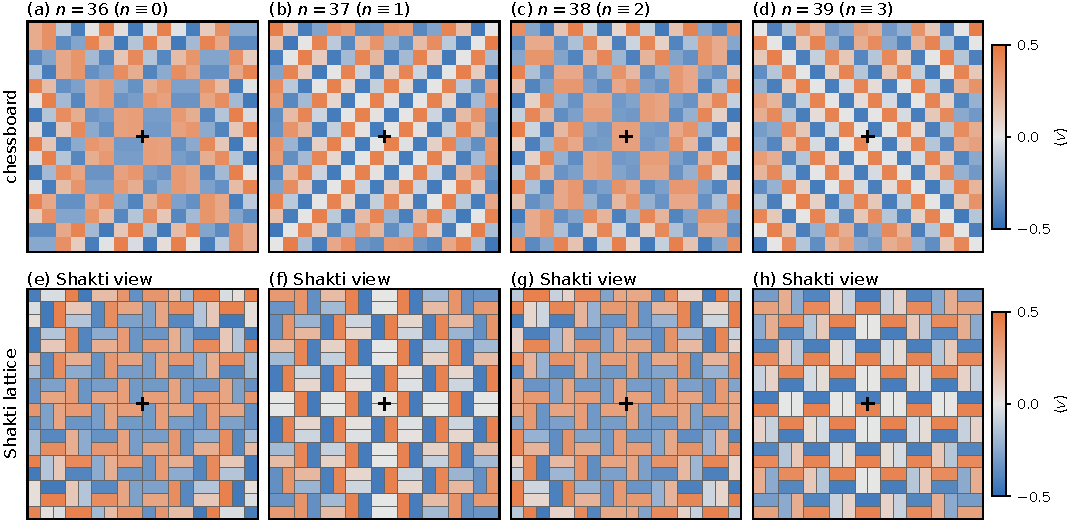
\includegraphics[width=\textwidth]{figs/fig4_exactmaps.pdf}
\caption{Exact vorticity pattern at the center of the Aztec diamond (placement I) for $n=36$--$39$, one size per residue class of $n\bmod4$, computed with the Kasteleyn method of Sec.~\ref{sec:exact} without sampling. (a)--(d) Chessboard view; (e)--(h) Shakti view, in which each plaquette is colored by $\langle v\rangle$. The cross marks the center. The $2\times2$ superstructure is present in every class; $n\bmod4$ decides whether it lives on the horizontal plaquettes ($n\equiv3$), the vertical plaquettes ($n\equiv1$), or both ($n$ even).}
\label{fig:exactmaps}
\end{figure*}

\subsection{Exact results}
\label{sec:exact}

Height differences are signed counts of crossed dominoes, and every crossing changes $h$ by 4 relative to the dimer-free increment. Therefore $\eps(p)=\eps_0(p)(-1)^{N_\gamma(p)}$, where $N_\gamma$ is the number of dominoes crossing a lattice path $\gamma$ from a boundary vertex to $p$ and $\eps_0$ is fixed by the geometry of the path. The expectation is a ratio of Kasteleyn determinants~\cite{Kasteleyn1961,Temperley1961},
\begin{equation}
\langle\eps(p)\rangle=\eps_0(p)\,\frac{\det K_\gamma}{\det K},
\label{eq:seam}
\end{equation}
where $K_\gamma$ is the Kasteleyn matrix with the edges crossing $\gamma$ negated. Domino-resolved averages $\langle v(d)\rangle$ follow from cofactors (Appendix~\ref{app:kasteleyn}). The method reproduces full enumeration at $n=4$ to machine precision and yields exact rational numbers with fraction-free elimination.

Three exact statements follow. First, $\langle\eps(\text{center})\rangle$ vanishes identically for $n\equiv1,2\pmod4$ (placement I), and the values for $n=4m-1$ and $n=4m$ coincide; this is the exact form of the orientation rule of Fig.~\ref{fig:exactmaps}. Second, the exact rationals have denominators $2^{2m(2m-1)}$ and numerators made of odd primes smaller than $4m$, which led us to the following closed form.

\begin{conjecture}[Central amplitude]
For the Aztec diamond of order $n=4m-1$ or $4m$ (placement I),
\begin{equation}
\bigl|\langle\eps(\text{center})\rangle\bigr|=2^{-2m(2m-1)}\prod_{\substack{j=1\\ j\ \text{odd}}}^{4m-1} j^{\,\min(4m-j,\;3j-4m)} .
\label{eq:product}
\end{equation}
\end{conjecture}

Equation~\eqref{eq:product} reproduces all exact rationals for $m=1$--8 (e.g.\ $3/4$, $3\cdot5^3\cdot7/2^{12}$, $3^3\cdot5^3\cdot7^5\cdot11/2^{30}$) and the floating-point Kasteleyn values up to $m=14$ within their numerical error. Third, its asymptotic expansion follows from Stirling's formula and the hyperfactorial expansion,
\begin{equation}
\ln\bigl|\langle\eps(\text{center})\rangle\bigr|=-\tfrac14\ln m+\tfrac14+\tfrac13\ln2-3\ln A+O(m^{-2}),
\label{eq:asym}
\end{equation}
with $A$ the Glaisher--Kinkelin constant. The central amplitude is therefore $C\,m^{-1/4}$ with $C=e^{1/4}2^{1/3}A^{-3}=0.76705\ldots$, in agreement with the extrapolated Kasteleyn data (Fig.~\ref{fig:exactscaling}). If Eq.~\eqref{eq:product} is proved---graphical condensation~\cite{Kuo2004} or symmetry factorization~\cite{Ciucu1997} are natural routes---the exponent $1/4$ at the sample center becomes a theorem that does not rely on the GFF limit.

\begin{figure*}[t]
\centering
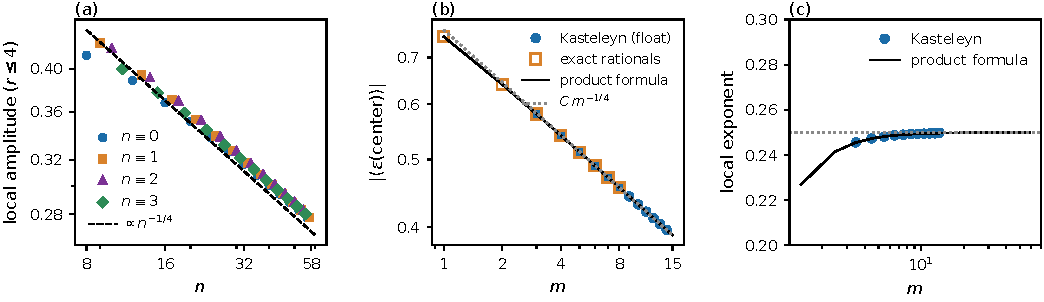
\includegraphics[width=\textwidth]{figs/fig5_exactscaling.pdf}
\caption{Exact amplitude of the vorticity order in the Aztec diamond. (a) Local amplitude (cells within distance 4 of the center) versus $n$ for the four residue classes, with the $n^{-1/4}$ law (dashed). (b) $|\langle\eps(\text{center})\rangle|$ for $n=4m-1$: floating-point Kasteleyn values (circles), exact rationals (squares), the product formula of Eq.~\eqref{eq:product} (line), and its asymptote $C\,m^{-1/4}$ from Eq.~\eqref{eq:asym} (dotted). (c) Local exponent $-d\ln|\langle\eps\rangle|/d\ln m$, which approaches $1/4$.}
\label{fig:exactscaling}
\end{figure*}

\subsection{Shape dependence}

For a general region the amplitude at position $z$ follows from $\mathrm{Var}\,h(z)\simeq g\ln[N\rho_D(z)]$, where $\rho_D$ is the conformal radius of the unit-scaled region $D$:
\begin{equation}
A(z)\simeq C_D\,[N\rho_D(z)]^{-1/4}.
\label{eq:amplaw}
\end{equation}
For a $W\times H$ rectangle the central conformal radius is $H\rho(W/H)$ with $\rho(1)=0.539$ and $\rho(\infty)=2/\pi$. The short side therefore sets the amplitude, and elongation reduces it by at most 4\%. Monte Carlo simulations of 21 rectangles from $8\times8$ to $128\times32$ confirm this (Fig.~\ref{fig:rect}); the global fit gives $A=0.82\,(H\rho)^{-0.24}$. Square boards have no frozen regions and a flat mean height, and their amplitude ($0.38$ at $L=48$, exponent $0.25\pm0.02$) is larger than in an Aztec diamond of comparable size.

\begin{figure}[t]
\centering
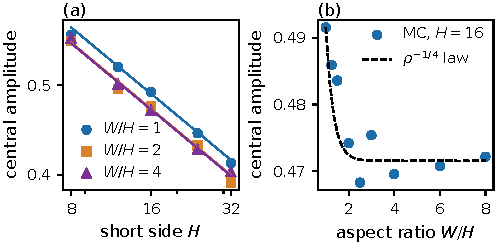
\includegraphics[width=\columnwidth]{figs/fig6_shape.pdf}
\caption{Shape dependence of the order (Monte Carlo, black corner). (a) Central amplitude versus the short side $H$ for aspect ratios $W/H=1$, 2, and 4; lines are the global fit $A=0.82\,(H\rho)^{-0.24}$. (b) Dependence on the aspect ratio at $H=16$, compared with the conformal-radius law of Eq.~\eqref{eq:amplaw}.}
\label{fig:rect}
\end{figure}

%==========================================================================
\section{Boundary control: the vorticity phase field}
\label{sec:phase}
%==========================================================================

\subsection{One field behind all patterns}

At a vertex $p$ one has $h\equiv r(p)\pmod4$, so $e^{i\pi h/4}=e^{i\pi r(p)/4}\eps(p)$ exactly. The four corners of a cell carry all four residues, which allows us to define a local complex order parameter,
\begin{equation}
\Psi(c)=\frac12\sum_{p\in\partial c}e^{i\pi r(p)/4}\langle\eps(p)\rangle,
\label{eq:psi}
\end{equation}
with the inverse relation
\begin{equation}
\langle v(d)\rangle=s(d)\,\mathrm{Re}\bigl[e^{-i\pi r(p_d)/4}\,\Psi\bigr].
\label{eq:projection}
\end{equation}
All vorticity patterns---for any size, placement, or shape---are thus projections of one slowly varying field $\Psi\simeq A\,e^{i\varphi}$. The modulus $A$ is the amplitude of Sec.~\ref{sec:order}; the phase $\varphi$ selects which sublattice of plaquettes carries the pattern and with which sign. Writing the central pattern as $\langle v\rangle\simeq2\,\mathrm{Re}[\alpha e^{i\pi(x+y)/2}+\beta e^{i\pi(x-y)/2}]$, one finds $\alpha$ real and $\beta$ imaginary, so $\alpha$ lives on the horizontal and $\beta$ on the vertical plaquettes. The pair $(\alpha,i\beta)$ is a two-component vector whose angle follows the phase of $\Psi$: shifting the mean height by 2 rotates it by $\pi/2$ and moves the order from one plaquette orientation to the other.

\subsection{Phase map}

For Gaussian fluctuations $\langle e^{i\pi h/4}\rangle=e^{i\pi\langle h\rangle/4}e^{-\pi^2\mathrm{Var}h/32}$, so the phase should be set by the mean height:
\begin{equation}
\arg\Psi(z)=\frac{\pi}{4}\,\langle h(z)\rangle .
\label{eq:phasemap}
\end{equation}
We tested Eq.~\eqref{eq:phasemap} against exact $\Psi$ with $\langle h\rangle$ computed exactly from the edge probabilities $K(b,w)K^{-1}(w,b)$ (Fig.~\ref{fig:phasemap}). On square and rectangular boards the rms phase error is $0.006$\,rad. In the Aztec diamond the relation is exact at the center, holds to better than $0.1$\,rad in the inner half of the liquid disk, and deviates by up to $0.3$\,rad only next to the arctic circle, where fluctuations are non-Gaussian. At large size $\langle h\rangle$ is the limit shape determined by the complex Burgers equation~\cite{Kenyon2007,KOS2006,Cohn1996}, so Eq.~\eqref{eq:phasemap} maps the variational limit shape directly onto the magnetic pattern. In the Aztec diamond the mean height is strongly curved, so the pattern rotates through all phases between the center and the frozen corners; in square boards the mean height is flat and the phase is uniform.

\begin{figure*}[t]
\centering
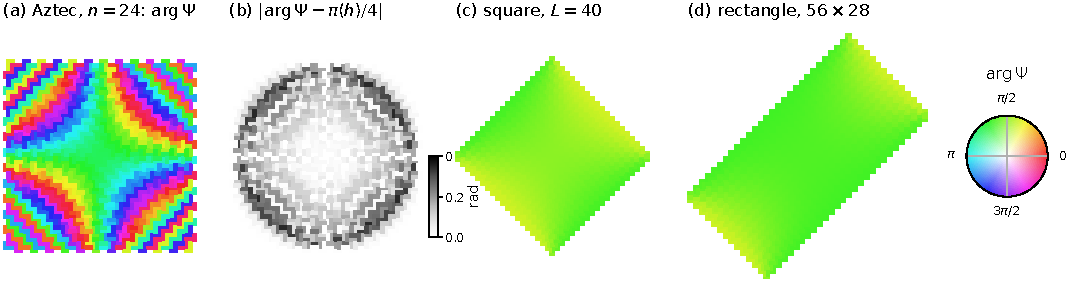
\includegraphics[width=\textwidth]{figs/fig7_phasemap.pdf}
\caption{Phase map. (a) Exact $\arg\Psi$ for the Aztec diamond with $n=24$ (placement I), shown on the Shakti plaquettes. (b) Absolute difference between $\arg\Psi$ and the prediction $\pi\langle h\rangle/4$ obtained from the exact mean height. (c), (d) Exact $\arg\Psi$ for a $40\times40$ square and a $56\times28$ rectangle; here the difference from $\pi\langle h\rangle/4$ is below 0.03\,rad everywhere (rms 0.006\,rad). The color wheel gives the phase.}
\label{fig:phasemap}
\end{figure*}

\subsection{The center is fixed by symmetry}

If a region is invariant under a $90^\circ$ rotation $R$ about a vertex $c$, $R$ exchanges the chessboard colors and therefore maps $h\to c_0-h$. The uniform measure is invariant, which gives the exact result
\begin{equation}
\langle h(c)\rangle=\tfrac12\bigl[h(p)+h(Rp)\bigr]
\label{eq:center}
\end{equation}
for any boundary vertex $p$. For the Aztec diamond, in the normalization $h=r$ at the bottom corner, this gives $\langle h(c)\rangle=3-n$ ($n$ even) and $1-n$ ($n$ odd) for placement I, and $n+2$ ($n$ even) and $n$ ($n$ odd) for placement II. We verified these integers with Kasteleyn calculations for $n=8$--40, and they agree with the exact central phases in Figs.~\ref{fig:psi}(a)--\ref{fig:psi}(d). Every mod-4 and placement rule then follows from $\langle h(c)\rangle$ (Table~\ref{tab:orient}): $\langle h(c)\rangle\equiv2\pmod4$ puts the order only on horizontal plaquettes, $\equiv0$ only on vertical plaquettes, and odd values on both with equal weight. Its value modulo 8 fixes the sign. The size of the sample modulo 4 and its placement on the lattice are therefore the design parameters that select the imprinted pattern.

\begin{table}[b]
\caption{Which plaquettes carry the central order. The rule follows from $\langle h(c)\rangle\bmod4$ [Eq.~\eqref{eq:center}] and is confirmed exactly for the Aztec diamond and by Monte Carlo for square boards.}
\label{tab:orient}
\begin{ruledtabular}
\begin{tabular}{lccc}
$\langle h(c)\rangle\bmod4$ & 2 & 0 & odd\\
Ordered plaquettes & horizontal & vertical & both\\
\hline
Aztec, placement I & $n\equiv3$ & $n\equiv1$ & $n$ even\\
Aztec, placement II & $n\equiv0$ & $n\equiv2$ & $n$ odd\\
Square board & black corner & -- & white corner\\
\end{tabular}
\end{ruledtabular}
\end{table}

\begin{figure*}[t]
\centering
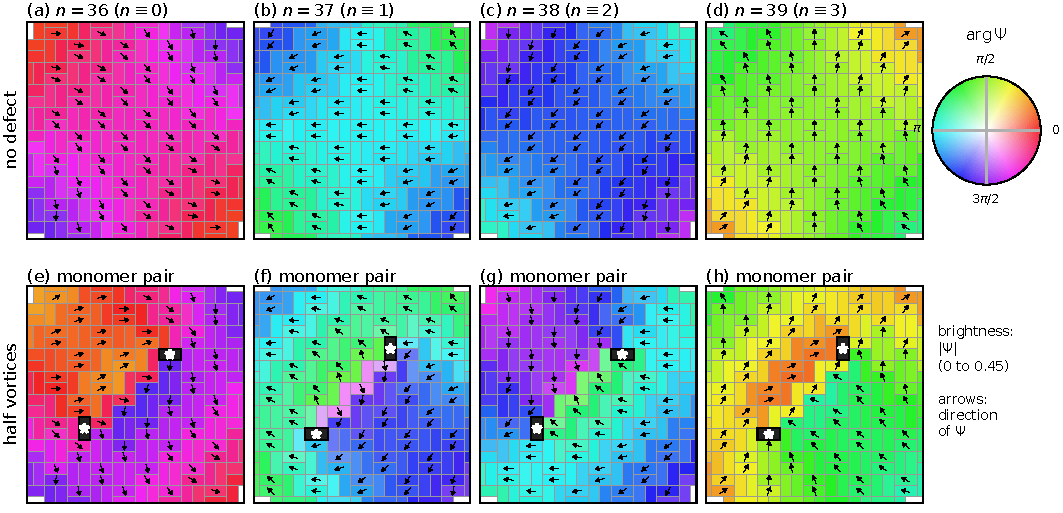
\includegraphics[width=\textwidth]{figs/fig8_psi_I.pdf}
\caption{Exact phase field $\Psi$ at the center of the Aztec diamond (placement I, $n=36$--39), shown on the Shakti plaquettes; hue is $\arg\Psi$, brightness $|\Psi|$, and arrows give the direction of $\Psi$. (a)--(d) Without defects the phase is uniform and changes with $n\bmod4$ as predicted by Eq.~\eqref{eq:center}. (e)--(h) With a pair of monomers (stars) seven cells apart, the phase winds by $\pi$ around each monomer and opposite hues meet along a line, the string (Sec.~\ref{sec:defects}).}
\label{fig:psi}
\end{figure*}

\subsection{Holes and pinned regions}
\label{sec:holes}

A central hole adds a second boundary whose rim vorticity is fixed up to a winding sector $k$ (a rim height offset $4k$). Kasteleyn calculations with a flux through the hole give the sector weights. For holes of size $H\equiv0\pmod4$ one sector dominates overwhelmingly (99.1\% for $H=8$ in an $L=48$ board), so the hole pins the pattern by itself. For $H\equiv2\pmod4$ two sectors have equal weight, and the rim vorticity is a free Ising variable that an external pinning field can select.

When the rim pattern agrees with the one imposed by the outer boundary, the order is reinforced: the local amplitude reaches $0.61$ at the rim, compared with $0.38$ without a hole [Figs.~\ref{fig:holes}(a) and \ref{fig:holes}(d)]. When the rim pattern is opposite, the order does not cancel. Instead $\Psi$ rotates by $\pi$ across the annulus while $|\Psi|$ stays unchanged, because the forcing moves only the mean height, not its fluctuations. Halfway through the twist the order is carried entirely by the other plaquette orientation. The twist follows the logarithmic interpolation of $\langle h\rangle$: the crossover ring is predicted at the geometric mean of the hole and sample radii ($9.8$ cells) and observed at $9$ cells. A pinned structure thus reinforces the imprinted pattern when aligned and produces a horizontal/vertical crossover ring when misaligned.

\begin{figure*}[t]
\centering
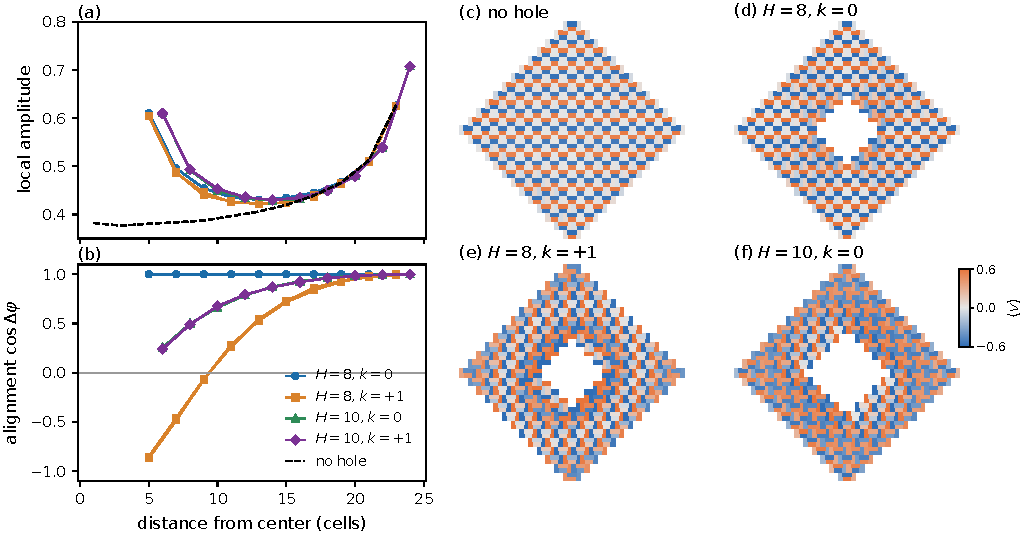
\includegraphics[width=\textwidth]{figs/fig9_holes.pdf}
\caption{Central holes in an $L=48$ square board (Monte Carlo in fixed winding sectors $k$). (a) Local superstructure amplitude and (b) alignment $\cos\Delta\varphi$ with the hole-free pattern versus distance from the center, for holes of size $H=8$ and 10. (c)--(f) $\langle v\rangle$ maps. In the natural sector ($k=0$) of the $H=8$ hole the pattern is reinforced; in the forced sector ($k=+1$) it twists by $\pi$ through a ring in which the other plaquette orientation carries the order. For $H=10$ the two sectors are degenerate.}
\label{fig:holes}
\end{figure*}

%==========================================================================
\section{Correlations and scattering signature}
\label{sec:corr}
%==========================================================================

The two-point function of the vorticity phase can also be computed exactly. With a seam running from $p$ to $q$,
\begin{equation}
G(p,q)=\bigl\langle e^{i\pi[h(q)-h(p)]/4}\bigr\rangle=e^{i\pi\Delta h_0/4}\,\frac{\det K_\gamma}{\det K},
\label{eq:twopoint}
\end{equation}
where $\Delta h_0$ is the dimer-free height increment along the seam. On square boards of size $L=32$, 64, and 96, $L^{1/2}|G(r)|$ collapses onto a single function of $r/L$ to within 1\% [Fig.~\ref{fig:corr}(a)]. This confirms the two-point exponent $2x=1/2$ without adjustable parameters. The collapse function is not the pure Dirichlet-GFF prediction (deviations of up to 15\%), reflecting the non-Temperleyan corners of an even board~\cite{Russkikh2018}; the exponent is unaffected.

In an experiment the natural observable is the structure factor. We computed $S(\bm q)=L^{-2}\langle|\sum_c v(c)e^{i\bm q\cdot\bm R_c}|^2\rangle$ for the vorticity field on the plaquette centers $\bm R_c$ (Shakti units, lattice constant $a=1$) with Monte Carlo for $L=32$--128 [Fig.~\ref{fig:corr}(b)--(d)]. Peaks appear at $\bm q_0=\pi(\pm\tfrac12,\pm1)$, $\pi(\pm1,\pm\tfrac12)$, $\pi(0,\pm\tfrac12)$, and weakly at $\pi(\pm\tfrac12,0)$, with relative weights set by the boundary. Algebraic order with exponent $x$ gives
\begin{equation}
S(\bm q_0+\bm k)=L^{2-2x}\,F(kL),\qquad F(u)\sim u^{-(2-2x)}\ (u\gg1),
\label{eq:sq}
\end{equation}
that is, peak heights $\propto L^{3/2}$ and tails $\propto|\bm q-\bm q_0|^{-3/2}$. The data give a peak-height exponent of $1.53$ and a scaling collapse with the $-3/2$ tail for $kL\lesssim12$. Such power-law superlattice peaks distinguish the vorticity order from true long-range order ($S\propto L^2$) and from short-range order ($S\propto L^0$). They sit at odd multiples of $\pi/4$ in the island-moment structure factor, between the Bragg positions of the bare Shakti lattice.

\begin{figure*}[t]
\centering
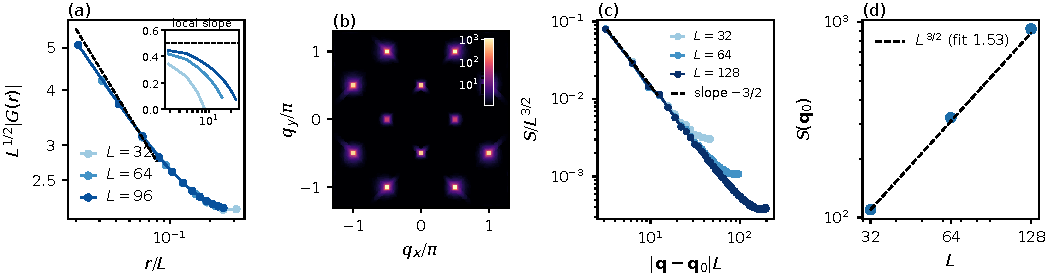
\includegraphics[width=\textwidth]{figs/fig10_corr.pdf}
\caption{Correlations and scattering. (a) Exact phase correlation on square boards: $L^{1/2}|G(r)|$ versus $r/L$ collapses for $L=32$--96; inset: the local slope approaches $1/2$. (b) Vorticity structure factor for $L=128$ (Monte Carlo, logarithmic color scale; peaks are widened by a $7$-pixel maximum filter for visibility). (c) Scaled peak profile $S/L^{3/2}$ versus $|\bm q-\bm q_0|L$ with the $-3/2$ tail. (d) Peak height versus $L$, with fitted slope 1.53.}
\label{fig:corr}
\end{figure*}

%==========================================================================
\section{Topological defects of the vorticity order}
\label{sec:defects}
%==========================================================================

Real arrays contain defects. Here we ask only how defects affect the vorticity order; where diagonal defects appear and how their density depends on temperature is the subject of a separate study~\cite{Won2026}. The relevant property of a point defect is its winding: going once around it, $h$ changes by $\Delta h$ and the phase $\theta=\pi h/4$ by $\pi\Delta h/4$. Since $\eps=(-1)^{\floor{h/4}}$ has period 8 in $h$, two classes arise.

\emph{Half vortices ($\Delta h=\pm4$) are confined.} The simplest example is a monomer, an uncovered plaquette. Around it $\Psi$ changes sign, so every loop of tetrominoes enclosing a monomer has coupling product $-1$. A string of violated couplings must therefore connect monomers to each other or to the free boundary [Figs.~\ref{fig:strings}(a) and \ref{fig:strings}(c)]. In the exact maps the string appears as a line along which opposite hues meet [Figs.~\ref{fig:psi}(e)--\ref{fig:psi}(h)]. The minimal number of violated couplings grows linearly with the separation, by about 1.25 per chessboard step [Fig.~\ref{fig:strings}(d)]. In a Shakti vertex model each violated coupling costs energy. With the unhappy vertices fixed by the tiling and all island spins optimized by integer programming, the excess energy of a monomer pair grows by one type-II $z=4$ vertex per diagonal step [Fig.~\ref{fig:strings}(e)]. In the plain dimer model monomers interact only logarithmically, $Z_{\rm pair}\propto r^{-1/2}$~\cite{Fisher1963} [Fig.~\ref{fig:strings}(f)]; in Shakti ice the string turns this into linear confinement. Half vortices can therefore neither unbind nor scramble the pattern: they either bind in pairs or are expelled to the sample edge.

\emph{Full vortices ($\Delta h=\pm8$) are free.} Around such a defect $\Psi$ winds by $\pm2\pi$ and returns to itself, so no coupling is violated and no string forms. The diagonal (O-tetromino) tiles, which cover a $2\times2$ Shakti block with a charge $\pm2$ at its center, belong to this class once the corner shared by their two cells is counted as part of the defect [Fig.~\ref{fig:strings}(b)]. Exact pair weights give $Z_{\rm pair}(r)/Z\propto r^{-2x_v}$ with $2x_v=2.05$, i.e.\ a scaling dimension $x_v=1$ [Fig.~\ref{fig:strings}(f)]. This is four times the half-vortex value, as expected for a doubled magnetic charge in a Coulomb gas~\cite{Nienhuis1987}. Since $x_v<2$, a finite density of free full vortices is relevant in the renormalization-group sense~\cite{Kosterlitz1973,Jose1977}: it cuts the algebraic order off beyond a screening length $\xi\sim y^{-1/(2-x_v)}=y^{-1}$, where $y$ is the defect fugacity. Full vortices thus screen the order rather than frustrate it.

\begin{figure*}[t]
\centering
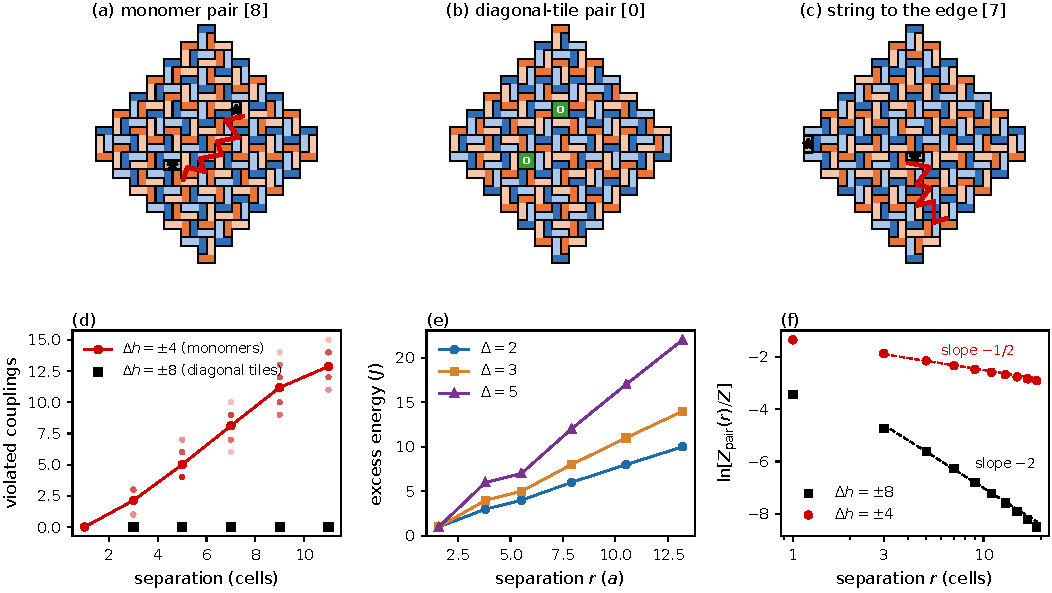
\includegraphics[width=\textwidth]{figs/fig11_strings.pdf}
\caption{Topological defects. (a)--(c) Single tilings of a $14\times14$ board with vorticities from the island rule; red segments mark a minimal set of violated couplings, whose number is given in brackets. (a) Two monomers (stars, half vortices) are joined by a string. (b) Two diagonal tiles (full vortices) cause no violated coupling. (c) A monomer near the center sends its string to the free boundary. (d) Minimal number of violated couplings versus separation ($22\times22$ board, eight tilings per point). (e) Shakti vertex model: excess energy of a monomer pair on a $24\times24$ torus for type-II and charged-vertex costs $\Delta=2$, 3, and 5, in units of the unhappy-vertex energy $J$. (f) Exact pair weights on a $64\times64$ board: $r^{-1/2}$ for half vortices and $r^{-2}$ for full vortices.}
\label{fig:strings}
\end{figure*}

%==========================================================================
\section{Dipolar interactions and temperature}
\label{sec:dipolar}
%==========================================================================

So far all ground states were weighted equally. In real arrays the long-range dipolar interaction lifts this degeneracy. Within the ground-state manifold every tiling fixes all island moments through the templates, so each tiling has a well-defined dipolar energy. We simulated this energy with Metropolis height flips on $L\times L$ boards ($L=24$--64). Moments were modeled either as point dipoles or as dumbbells of length $0.7a$, with a cutoff of $6a$ (results unchanged at $10a$), in units of $D=\mu_0m^2/4\pi a^3$. A flip changes only the two flipped tetrominoes, so updates are local. The cheapest excitation out of the manifold costs at least $3.8D$ (point) or $7.5D$ (dumbbell), far above the scales found below; restricting to the manifold is therefore justified. This realizes a two-stage ordering, familiar from dipolar kagome ice~\cite{Chern2011}: vertex frustration first, then selection within the degenerate manifold.

The results are summarized in Fig.~\ref{fig:dipolar}. Above $T\approx0.6D$ the effective exponent is unchanged within errors: the algebraic phase and all boundary-control results of Sec.~\ref{sec:phase} survive. On approaching $T_c\approx0.45D$ the height field stiffens ($2x$ drops to about $0.4$), and at $T_c$ the specific heat peaks. Below $T_c$ the tiling locks into a flat crystal with wave vector $(\pi/2,\pi/2)$ in chessboard coordinates, which is neither columnar nor staggered. In this crystal every tetromino has a fixed vorticity ($|\langle v\rangle|=1$): the algebraic order of the degenerate manifold turns into true long-range vorticity order. The dumbbell model gives the same crystal at a similar $T_c$, in the spirit of interacting-dimer models whose height field locks at low temperature~\cite{Alet2005}. Because the crystal has several degenerate variants with different locked heights, a boundary-selected phase [Eq.~\eqref{eq:center}] incompatible with the crystal produces grain boundaries, one of which is visible in Fig.~\ref{fig:dipolar}(h) at $T=0.3D$.

The full vortices of Sec.~\ref{sec:defects} remain the only defects that can compete with the order in this window. How many of them appear at a given temperature depends on their creation energy, which is sensitive to the short-range form of the interaction and hence to island shape and gaps; this question is addressed in Ref.~\cite{Won2026}.

\begin{figure*}[t]
\centering
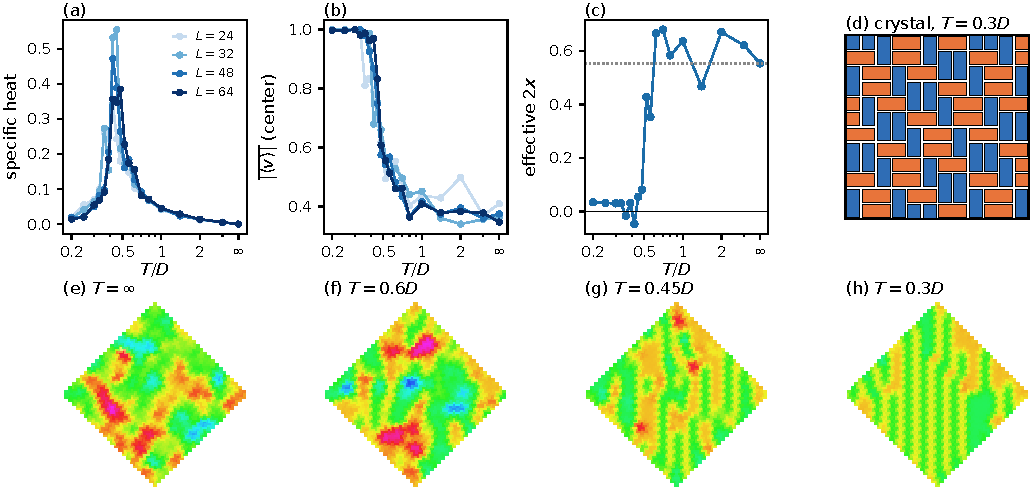
\includegraphics[width=\textwidth]{figs/fig12_dipolar.pdf}
\caption{Dipolar interactions within the ground-state manifold (point dipoles, $L\times L$ boards). (a) Specific heat per cell. (b) Mean $|\langle v\rangle|$ in the central window: algebraic order above $T_c\approx0.45D$ and long-range order ($|\langle v\rangle|=1$) below. (c) Effective exponent $2x$ from the finite-size scaling of $\langle|\bar\Psi|^2\rangle$ over $L=24$--64; the dotted line is the $T=\infty$ estimate at these sizes. (d) Low-temperature crystal in the chessboard view. (e)--(h) Phase field of single states at $L=48$ (color wheel as in Fig.~\ref{fig:psi}); a grain boundary is visible at $T=0.3D$.}
\label{fig:dipolar}
\end{figure*}

%==========================================================================
\section{Implications for experiments}
\label{sec:design}
%==========================================================================

The results translate into a small set of rules for designing and reading out vorticity order in Shakti arrays.

\emph{Where the order lives.} The algebraic order fills the liquid region. Square and rectangular samples are liquid throughout; an Aztec-diamond boundary confines it to a central disk of radius $n/\sqrt2$ cells and freezes the corners.

\emph{Which pattern.} The phase of the pattern is $\pi\langle h\rangle/4$. For $90^\circ$-symmetric samples the center is fixed exactly by Eq.~\eqref{eq:center}. Sample size modulo 4 and placement select horizontal-only, vertical-only, or mixed order (Table~\ref{tab:orient}). Increasing $n$ by one shifts the central phase alternately by $-3\pi/4$ and $+\pi/4$ (placement I) or by $-\pi/4$ and $+3\pi/4$ (placement II).

\emph{Net vorticity.} $V$ is fixed by the boundary [Eq.~\eqref{eq:Vboundary}]. Samples with $V=\pm2$ carry a net circulation regardless of the internal state.

\emph{How strong.} The amplitude decays only as $(\text{size})^{-1/4}$; it is about 0.4 at the center of an Aztec diamond with $n\approx40$. Compact shapes with a large conformal radius maximize it. Resolving $\langle v\rangle\approx0.4$ to 10\% on one plaquette requires about 600 independent images, fewer if symmetry-equivalent plaquettes are averaged.

\emph{Pinning.} Holes of size $\equiv0\pmod4$ pin their rim; holes of size $\equiv2\pmod4$ act as switchable Ising elements. Aligned pinning reinforces the pattern, while misaligned pinning creates a crossover ring at the geometric mean of the two radii.

\emph{Temperature window and defects.} Algebraic order is expected for $T_c\approx0.45D<T\ll$ vertex gap (4--8$D$), and long-range order below $T_c$ if the dynamics allow it. Half vortices are confined in any case; only free full vortices limit the order, through the screening length set by their density.

\emph{Read-out.} In real space each image can be demodulated into $\Psi$ via Eq.~\eqref{eq:psi}: uniform color indicates order, pinwheels mark full vortices, and color jumps along lines mark the strings attached to half vortices. In reciprocal space the order appears as power-law peaks at $\bm q_0$ with heights $\propto L^{3/2}$.

%==========================================================================
\section{Conclusions}
\label{sec:conclusion}
%==========================================================================

We have shown that the degenerate ground states of Shakti artificial spin ice host a hidden collective order: the vorticity of the L-tetrominoes formed by unhappy vertices and their plaquettes. Far from being an independent Ising variable, this vorticity is a nonlocal functional of the dimer configuration, $v=s(-1)^{\floor{h/4}}$. Three physical consequences stand out. First, the total vorticity is a topological invariant fixed by the sample boundary, for which we derived a closed formula. Second, the vorticity displays algebraic order with the exact exponent $1/4$, imprinted by the boundary into the bulk; its amplitude at the Aztec center appears to follow a closed product formula with the constant $e^{1/4}2^{1/3}A^{-3}$. Third, a single phase field $\Psi\simeq e^{i\pi\langle h\rangle/4}$, set by the dimer limit shape, organizes all patterns, so that sample size, placement, holes, and pinning become knobs that select and rotate the magnetic texture. Point defects fall into two topological classes: half vortices are confined by strings, while full vortices are free and screen the order. Dipolar interactions preserve the algebraic phase over a wide temperature window and eventually lock it into long-range order.

These results turn the abstract height field of the dimer model into a directly observable magnetic texture and offer a new way to use boundaries as a design tool in artificial spin ice. Several questions remain open: a proof of the product formula~\eqref{eq:product}; the universality class and variants of the dipolar locking transition, including realistic island shapes and kinetics; and whether analogous vorticity orders exist in other vertex-frustrated geometries. For Tetris ice, whose ground states reduce to one-dimensional structures~\cite{Gilbert2016}, and Santa Fe ice, whose unhappy vertices form strings~\cite{Zhang2021}, we expect at most short-range vorticity correlations, which singles out Shakti as the geometry with a two-dimensional height field. The recent observation of memory effects from topological constraints in Shakti ice~\cite{Priyanka2025} suggests that the vorticity may also be a useful variable for nonequilibrium studies.

\begin{acknowledgments}
[Acknowledgments and funding information to be added.]
\end{acknowledgments}

\section*{Data availability}
The data and computer codes that support the findings of this article are available from the author upon reasonable request.

\appendix

%==========================================================================
\section{Proofs}
\label{app:proofs}
%==========================================================================

\emph{The map.} Shakti unit squares are $[p,p+1]\times[q,q+1]$, and the block $(a,b)=[2a,2a+2]\times[2b,2b+2]$ is horizontal if $a+b$ is even. The cells of one fundamental domain map as follows: $(0,0)\mapsto$ squares $(0,1),(1,1)$ [H]; $(1,0)\mapsto(1,2),(1,3)$ [V]; $(1,1)\mapsto(0,4),(1,4)$ [H]; $(2,0)\mapsto(2,3),(3,3)$ [H]; $(1,-1)\mapsto(2,2),(3,2)$ [H]; $(2,1)\mapsto(2,4),(2,5)$ [V]; $(2,-1)\mapsto(4,2),(4,3)$ [V]; $(3,0)\mapsto(3,4),(3,5)$ [V]. All other cells follow by the translations $(2,2)\mapsto(0,4)$ and $(2,-2)\mapsto(4,0)$.

\emph{Island rule.} A shared island lies on the common boundary of plaquettes that belong to different tetrominoes. A counterclockwise circulation of one traverses that edge opposite to a counterclockwise circulation of the other. Agreement of the island orientation therefore requires opposite vorticities, with one sign change if the island is the defect island of exactly one of the tiles.

\begin{lemma}[Locality]\label{lem:local}
In any tiling of any simply connected region, Eq.~\eqref{eq:vformula} satisfies every island coupling.
\end{lemma}
\begin{proof}
Every coupled pair of dominoes $a,b$ shares a chessboard vertex. Edges on the perimeter of a domino are never crossed by a domino, so $h$ can be carried from $p_a$ along the perimeter of $a$ to the shared vertex and along the perimeter of $b$ to $p_b$. The difference $h(p_b)-h(p_a)$ is therefore a dimer-free increment that depends only on the relative placement of $a$ and $b$. The coupling sign also depends only on that placement. Shifting $h$ by 4 flips both $\eps$ factors, so $v(a)v(b)$ depends only on the relative placement and the position modulo 4. All 704 coupled placements (both orientations, 16 positions) were evaluated and satisfy the rule. Since this list is complete, the check is a proof.
\end{proof}

\emph{Connectivity.} The template fixes all ten perimeter islands of a tetromino. Two chess-adjacent cells map to plaquettes that share exactly one unit edge (verified on one period of the map); that edge separates different plaquettes, so it is an island. Edge-adjacent dominoes therefore share a prescribed island and are coupled. In a connected region any two dominoes are joined by a chain of edge-adjacent dominoes, so the coupling graph is connected and $v$ is unique up to a global sign.

\emph{Flip invariance.} A flip at block center $c$ changes only $h(c)$, by $\pm4$, and $c$ is the reference vertex of no domino. The flipped dominoes use the reference vertices $a=c-(1,1)$ together with $b=c-(1,0)$ (horizontal pair) or $d=c-(0,1)$ (vertical pair). The left and bottom block edges are never crossed, so $h(b)$ and $h(d)$ follow from $h(a)$ by one step. The block vorticity is thus a function of $(c\bmod4,\ h(a)\bmod8)$; evaluating Eqs.~\eqref{eq:vformula}--\eqref{eq:sfactor} in all 32 cases shows that it is unchanged by the flip (Fig.~\ref{fig:flip}).

\begin{figure}[t]
\centering
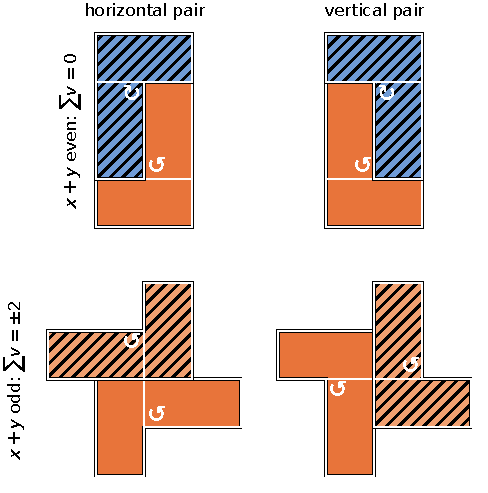
\includegraphics[width=\columnwidth]{figs/fig_flip.pdf}
\caption{Flip invariance in the Shakti view. Upper row: blocks whose lower-left cell has $x+y$ even carry opposite vorticities in both fillings ($\sum v=0$). Lower row: blocks with $x+y$ odd carry equal vorticities of the same sign in both fillings ($\sum v=\pm2$). Hatching distinguishes the two tetrominoes; one representative sign choice is shown.}
\label{fig:flip}
\end{figure}

\emph{Boundary formula.} In the brick tiling the lattice line under each row is never crossed, so $h(x+2,y)=h(x,y)$ along it, while $s_{\rm H}(x+2,y)=-s_{\rm H}(x,y)$ by Eq.~\eqref{eq:sfactor}. Consecutive bricks cancel, rows of length $\equiv0\pmod4$ contribute nothing, and rows of length $\equiv2\pmod 4$ contribute the vorticity of their first brick, which gives Eq.~\eqref{eq:Vboundary}.

\emph{Center height.} The $90^\circ$ rotation $R$ about $c$ maps cell $(i,j)$ to a cell of the opposite color, so the height of the rotated tiling is $c_0-h\circ R^{-1}$. Invariance of the uniform measure gives $\langle h(c)\rangle=c_0-\langle h(c)\rangle$, and $c_0=h(p)+h(Rp)$ for any boundary vertex $p$.

%==========================================================================
\section{Kasteleyn methods}
\label{app:kasteleyn}
%==========================================================================

We use the Kasteleyn matrix $K$ with weights 1 (horizontal) and $i$ (vertical) between black and white cells~\cite{Kasteleyn1961,KenyonLectures}; for exact rational arithmetic, an equivalent real signing is combined with fraction-free (Bareiss) elimination. $\langle\eps(p)\rangle$ follows from Eq.~\eqref{eq:seam} with the seam flips placed on the edges crossed by a breadth-first lattice path. For a domino $d$ covering the black cell $b$ (row index $i$ of $K$) and the white cell $w$ (column index $j$), $\langle\mathbb 1_d\,\eps(p_d)\rangle=\eps_0K_\gamma(b,w)(-1)^{i+j}\det K_\gamma^{(bw)}/\det K$, where $\mathbb 1_d$ indicates that $d$ is present and $K_\gamma^{(bw)}$ is the minor without row $i$ and column $j$; this form also covers the cases in which $\det K_\gamma=0$.

\emph{Holes and defects.} For diagonal tiles the corresponding cells are removed and the shared corner of each diagonal tile is excluded from the paths. For a pair of monomers the single-cell holes violate the Kasteleyn condition; negating the edges crossed by a dual path between the two holes restores it, and a straight branch cut between the monomers is excluded from the seam paths. All cases were validated against brute-force enumeration (pairs of diagonal tiles at $n=4$--6, monomer pairs at $n=5$ and 6) to about $10^{-15}$. Pair weights $Z_{\rm pair}(r)/Z$ are ratios of determinants with and without the holes. The mean height follows from the edge probabilities $P(b,w)=K(b,w)K^{-1}(w,b)$ integrated along paths. The two-point function uses a seam from $p$ to $q$ [Eq.~\eqref{eq:twopoint}]. Double precision is sufficient up to $n\approx58$ for the Aztec diamond; the exact rationals were obtained up to $n=31$.

%==========================================================================
\section{Simulations}
\label{app:sim}
%==========================================================================

Uniform Aztec-diamond tilings were generated by domino shuffling ($n\le195$, $10^3$--$2\times10^3$ tilings per size), and square and rectangular boards by height-function Metropolis flips (burn-in $20L^2$ sweeps, measurements spaced by $L^2/16$ sweeps, four independent replicas). Structure factors were computed by fast Fourier transform of $v$ placed on the plaquette centers. Dipolar simulations used Metropolis flips whose energy change was evaluated from the template spins of the two flipped tetrominoes with precomputed neighbor lists; the accumulated energy was checked against full recomputation. String lengths were obtained by integer linear programming of the minimal number of violated couplings, and vertex-model energies by integer programming over all island spins with vertex-type costs (unhappy $z=3$: 1; type-II and charged $z=4$, charged $z=2$ and $|q|=3$ $z=3$ vertices: $\Delta$).

\bibliography{refs}

\end{document}
